\documentclass[12pt]{article}
\usepackage[utf8]{inputenc}
\newcommand\preamble{
    \usepackage[italian]{babel}
    \usepackage{geometry}
    \usepackage{amsmath}
    \usepackage{amssymb}
    \usepackage{graphicx}
    \usepackage{ulem}
    \usepackage[dvipsnames]{xcolor}

    \geometry{margin=2cm}
    \let\olditemize\itemize
    \renewcommand\itemize{\olditemize\setlength\itemsep{0em}}
    \graphicspath{{../Immagini/}}

    \author{Lorenzo Vaccarecci}
}
\preamble

\title{Ottimizzazione Fisica (Parte 3)}
\date{7 Maggio 2024}

\begin{document}
\maketitle
\begin{lstlisting}[language=SQL]
    SELECT *
    FROM Noleggi N, Video V, Film F
    WHERE N.colloc = V.colloc AND
    V.titolo = F.titolo AND
    V.regista = F.regista 
\end{lstlisting}
Il risultato del join tra Noleggi e Video deve essere memorizzato nel buffer se ci sta, altrimenti su disco.
\section{Pipeline}
Si può applicare solo se \remark{l’operatore fisico esegue un ciclo sulla relazione outer}. Non tutti gli algoritmi possono essere eseguiti in pipeline:
\begin{itemize}
    \item Nested loop semplice
    \item Nested loop a blocchi
    \item Indexed nested loop
\end{itemize}
n questo caso,\important{il pipeline viene applicato alla relazione outer
mentre la relazione inner, utilizzata ad ogni ciclo per i confronti,
deve essere materializzata}
\begin{center}
    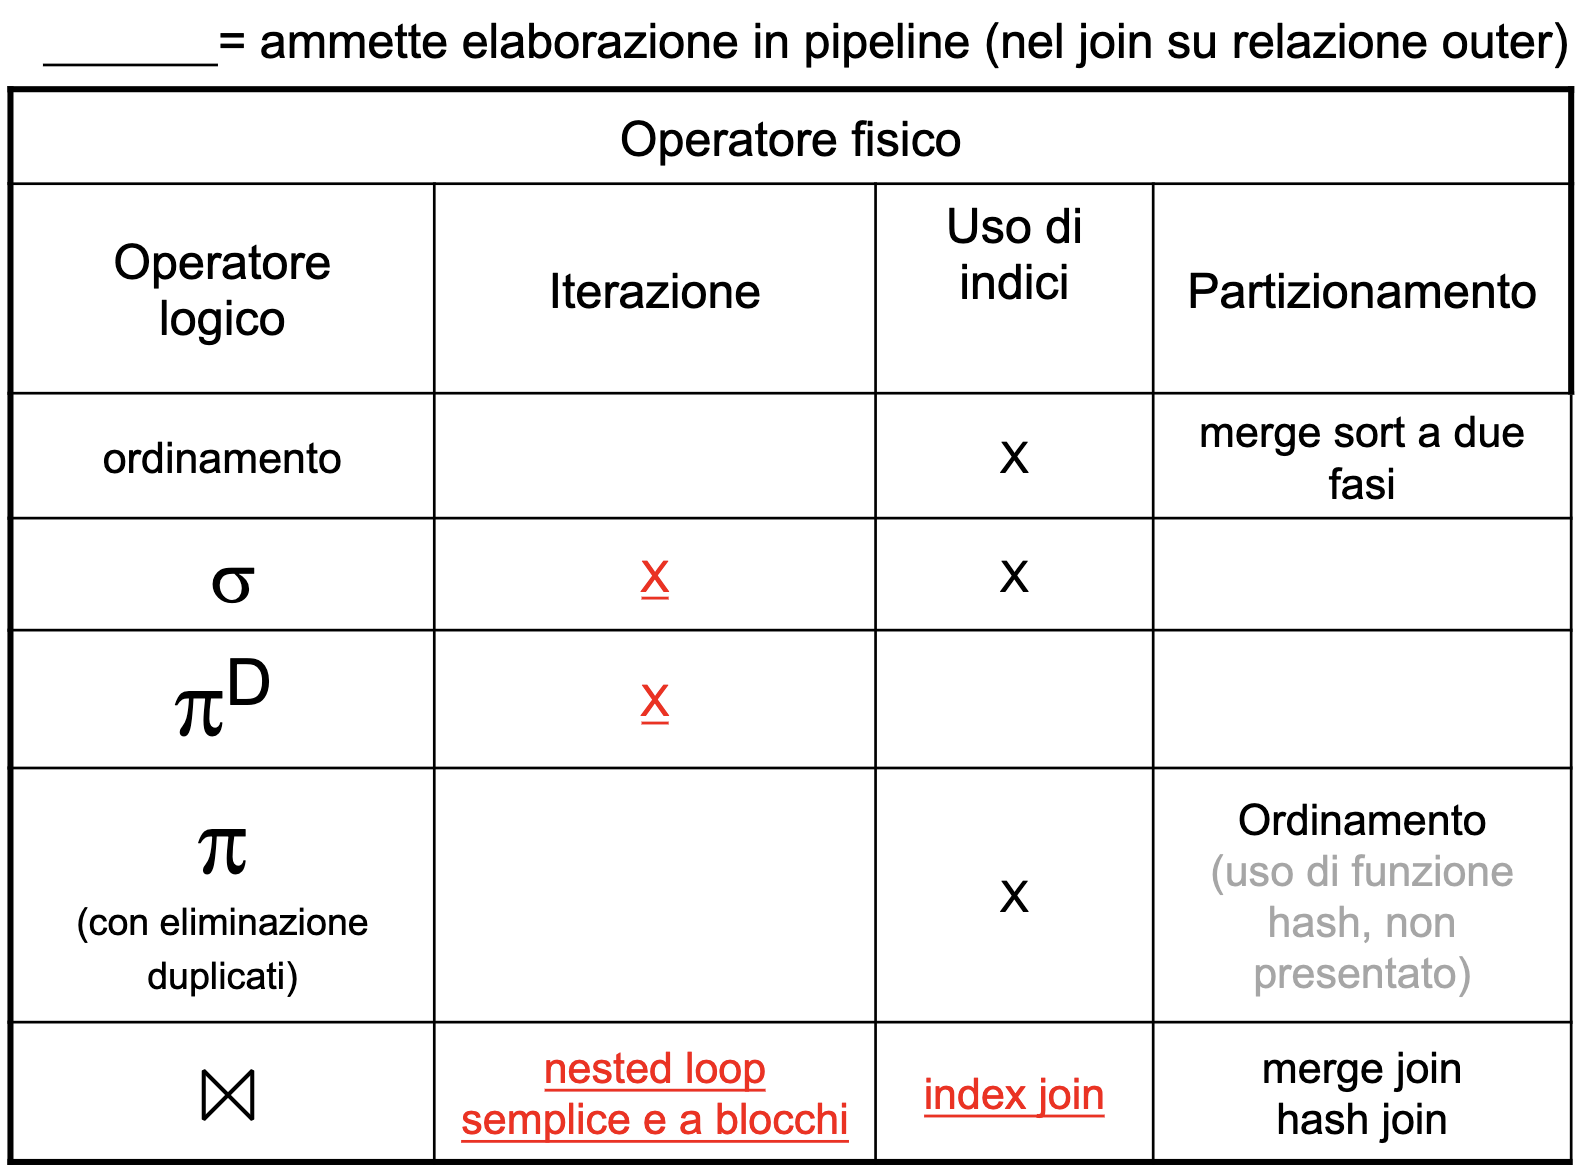
\includegraphics[scale=0.4]{pipeliningOpFisici.png}
\end{center}
\section{Stima del costo di un piano di esecuzione}
Per ogni piano, la stima viene fatta a partire dalle foglie (\remark{bottom-up}). Per stimare il costo di un piano di esecuzione vengono considerati i \important{costi di accesso} e per ogni nodo dell'albero il \important{costo dell'operazione} e la \important{dimensione del risultato}. Il tutto poi sommato.\\
Le statistiche non sono sempre aggiornate, infatti sono aggiornate periodicamente. Molti DBMS prevedono un comando per richiedere l'aggiornamento delle statistiche (\texttt{ANALYZE} in PostgreSQL).
\subsection{Esempio di stima del costo: Selezione}
\Tree [ .$\sigma_{R.C=3}$ [ .$\Join$ R S ] ]\\
Il numero di tuple restituito è dipende da quante tuple di $R$ soddisfano la condizione (P).\\
\important{Fattore di selettività: F(P)}, se è $<1$ è molto selettivo (poche tuple che soddisfano P) e viceversa.\\
\question{Quante sono le tuple restituite da $\sigma_{P}(R)$?}
$F(P)\cdot T(R)$\\
\question{Come si stima il fattore di selettività?}
$F(P)=\frac{\text{Casi favorevoli}}{\text{Casi possibili}}=\frac{1}{V(C,R)}$, a numeratore c'è il numero di valori della condizione. (\textit{Più formule nelle slide p.63})
\section{Euristica per join}

\subsection{Piano Left Deep}
\begin{equation*}
    R \Join S \Join T \Join V
\end{equation*}
\Tree[ .$\Join$ [ .$\Join$ [ .$\Join$ R S ] T ] V ]
\Tree[ .$\Join$ [ .$\Join$ R S ] [ .$\Join$ T V ] ]\\
L'albero di sinistra è Left Deep, quello di destra no.
\subsection{Progettazione Fisica}
\important{Dato un carico di lavoro, l’attività di progettazione fisico si
preoccupare di progettare uno schema fisico, in termini di
insieme di indici creati, che permetta di rendere il più possibile
efficiente l’esecuzione delle operazioni contenute nel workload}. Una scelta impropria degli indici può portare a:
\begin{itemize}
    \item inutilizzo degli indici
    \item scansioni sequenziali per uno o pochi record
    \item join multipli con tempi di esecuzione elevatissimi
    \item spreco di spazio disco1
\end{itemize}
\subsubsection{Approccio generale}
Si considerano uno alla volta le interrogazioni, partendo da quelle usate più frequentemente. Per ogni interrogazione $Q$:
\begin{itemize}
    \item si ipotizza un potenziale piano di esecuzione ottimale
    \item si individuano gli indici che permettono al sistema di prendere in considerazione il piano individuato
    \item si valuta empiricamente l'efficacia degli indici creati
    \item se gli indici non sono efficaci, cercare di comprendere la motivazione ed eventualmente rimuoverli dal livello fisico
\end{itemize}
Poi si valuta se gli indici identificati al passo i (per la
query $Q_{i}$) sono compatibili con gli indici
identificati fino al passo i-1 (per la query $Q_{i-1}$), ed
eventualmente si apportano correttivi, \textbf{solo un indice per relazione può essere clusterizzato}.
\end{document}